\section{Cônicas}


\subsection*{Completamento de Quadrados}


\begin{frame}[label=comp]
	\frametitle{Completamento de Quadrados}
	%\begin{scriptsize}
	
\begin{block}{Produto Notáveis}
	\[(x+k)^2=x^2+2k\cdot x+k^2\]
	\[(x-k)^2=x^2-2k\cdot x+k^2\]
\end{block}	

\begin{exe}
	Resolva as seguintes equações sem usar a fórmula de Bhaskara
	\begin{multicols}{2}
		\begin{enumerate}
			\item $x^2-x=0$
			\item $4x^2-1=0$
			\item $x^2-2x=8$
			\item $x^2-8x=9$
		\end{enumerate}
	\end{multicols}
	\medskip
\end{exe}

\end{frame}


\begin{frame}[label=comp]
	\begin{exe}
Complete os quadrados:
\begin{enumerate}
	\item $x^2+7x$
	\item $-2x^2+8x$
\end{enumerate}
	\end{exe}

\begin{block}{Fórmula de Bhaskara}
	Sejam  $a,b$ e $c\in\R$ com $a\neq 0$. Então as soluções da equação $ax^2+bx+c=0$ são dadas por
	\[ x=\frac{-b\pm \sqrt{b^2-4ac}}{2a}\]
\end{block}
\end{frame}

\begin{frame}[label=comp]
	
\begin{casa}
	Complete os quadrados:
\begin{enumerate}
	\item $x^2-4x$
	\item $-x^2+2x$
	\item $3x^2-9x$
\end{enumerate}
\end{casa}

\end{frame}

\subsection*{Elipse}

\begin{frame}[label=conicas]
	\frametitle{Elipse}
	%\begin{scriptsize}
	\uncover<1->{\begin{defin}[Elipse]
			Dados dois pontos no plano $F_1$ e $F_2$ uma \dest{elipse} é o lugar geométrico dos pontos do plano cuja soma das distâncias aos pontos $F_1$ e $F_2$ é constante. Os pontos $F_1$ e $F_2$ são chamados \dest{focos} da elipse.
		\end{defin}
	}

\begin{center}
	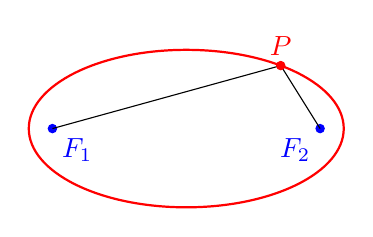
\begin{tikzpicture}
   \draw[thick,red] (0,0) ellipse (2cm and 1cm);
   \draw[fill,blue] (1.7,0) circle (1.5pt);
   \draw[fill,blue] (-1.7,0) circle (1.5pt);   
   \node[below left,blue] at (1.7,0) {$F_2$};
   \node[below right,blue] at (-1.7,0) {$F_1$};
   \node[above,red] at (1.2,0.8) {$P$};
 
   \draw (-1.7,0) -- (1.2,0.8) --(1.7,0);
     \draw[fill,red] (1.2,0.8) circle (1.5pt);
\end{tikzpicture}
\end{center}
\end{frame}


\begin{frame}[label=conicas]{Notação}
\begin{minipage}{0.4\textwidth}
	\begin{itemize}
	\item<1-> $F_1, F_2$: focos
		\item<2-> $F_1F_2$: segmento focal
		\item<3-> $O$: centro da elipse
		\item<5-> $A_1,A_2,B_1,B_2:$ Vértices
		
		\item<6-> $A_1A_2$: Eixo maior
		
		\item<7-> $B_1B_2$: Eixo menor
		
		\item<8-> $d(F_1,F_2)$: amplitude focal
	\end{itemize}
\end{minipage}
\begin{minipage}{0.4\textwidth}
	\begin{center}
		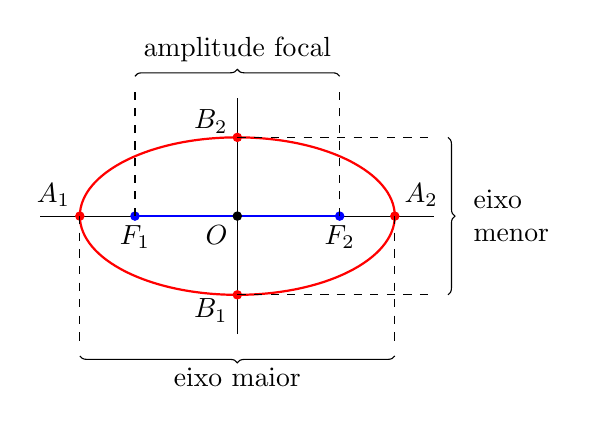
\begin{tikzpicture}
\uncover<2->{		\draw (-2.5,0) -- (2.5,0);
				\draw[thick,blue] (-1.3,0)--(1.3,0);  }
\uncover<4->{	\draw (0,-1.5) -- (0,1.5);}
%		\node[below right] at (2.5,0) {$x$};
%		\node[above left] at (0,1.5) {$y$};		
\uncover<1->{	\draw[thick,red] (0,0) ellipse (2cm and 1cm);}
\uncover<1->{		\draw[fill,blue] (1.3,0) circle (1.5pt);
		\draw[fill,blue] (-1.3,0) circle (1.5pt);   
	\node[below] at (1.3,0) {$F_2$};
		%	\node[below right,blue] at (-1.7,0) {$F_1$};
		\node[below] at (-1.3,0) {$F_1$};}
\uncover<5->{\draw[fill,red] (2,0) circle (1.5pt);   	
		\draw[fill,red] (-2,0) circle (1.5pt);
		\draw[fill,red] (0,1) circle (1.5pt);   	
		\draw[fill,red] (0,-1) circle (1.5pt);
		\node[above right] at (2,0) {$A_2$};
		\node[above left] at (-2,0) {$A_1$};
		\node[left] at (0,1.2) {$B_2$};
		\node[left] at (0,-1.2) {$B_1$};}
\uncover<3->{		\node[below left] at (0,0) {$O$};
		\draw[fill] (0,0) circle (1.5pt);}
		%	\draw (0,1) -- (1.3,0);
\uncover<6->{\draw[decoration={brace,mirror,raise=5pt},decorate] (-2,-1.6)--(2,-1.6);
			\draw[dashed] (-2,0) -- (-2,-1.6);
		\draw[dashed] (2,0) -- (2,-1.6); 
	\node[below] at (0,-1.8) {eixo maior};}	
\uncover<7->{\draw[decoration={brace,mirror,raise=5pt},decorate] (2.5,-1)--(2.5,1);
	\draw[dashed] (0,-1) -- (2.5,-1);
	\draw[dashed] (0,1) -- (2.5,1);
	\node[text width=1.cm] at (3.5,0) {eixo  menor};}

\uncover<8->{\draw[decoration={brace,raise=5pt},decorate] (-1.3,1.6)--(1.3,1.6);
\draw[dashed] (-1.3,0) -- (-1.3,1.6);
\draw[dashed] (1.3,0) -- (1.3,1.6); 
\node[below] at (0,2.4) {amplitude focal};}		

	
		
		%	\node at (-5,2) {$A_1,A_2,B_1,B_2:$ Vétices};
		
		%\node[above,red] at (1.2,0.8) {$P$};
		
		%\draw (-1.7,0) -- (1.2,0.8) --(1.7,0);
		%\draw[fill,red] (1.2,0.8) circle (1.5pt);
		\end{tikzpicture}
	\end{center}
\end{minipage}

	%\end{scriptsize}
\end{frame}


\begin{frame}[label=conicas]
	\uncover<1->{\begin{block}{}
			Dado uma elipse, considere um sistema de eixos cartesianos com eixo $OX$ determinado segmento focal, com origem no centro da elipse. Neste caso, sendo $2c$ a amplitude focal,  $2a$  a soma das distâncias de um ponto qualquer da elipse aos focos e $b^2=a^2-c^2$, então a equação da elipse é dada por
			
			\begin{center}
				\textcolor{red}{\fbox{$\displaystyle\frac{x^2}{a^2}+\frac{y^2}{b^2}=1$}}
			\end{center}
		A razão $e=\frac{c}{a}$ é chamada \dest{excentricidade da elipse} e, no caso, mede o achatamento da elipse. 
	\end{block}}


	\begin{center}
	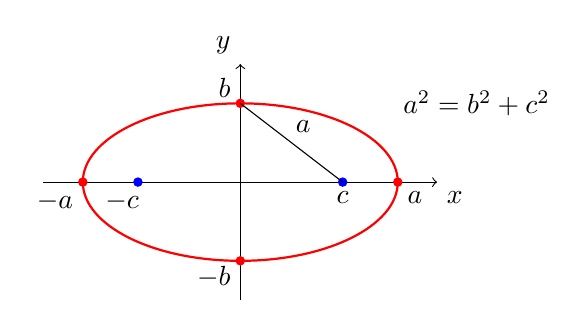
\begin{tikzpicture}
	\draw[->] (-2.5,0) -- (2.5,0);
	\draw[->] (0,-1.5) -- (0,1.5);
	\node[below right] at (2.5,0) {$x$};
	\node[above left] at (0,1.5) {$y$};		
	\draw[thick,red] (0,0) ellipse (2cm and 1cm);
	\draw[fill,blue] (1.3,0) circle (1.5pt);
	\draw[fill,blue] (-1.3,0) circle (1.5pt);   
	\node[below] at (1.3,0) {$c$};
	%	\node[below right,blue] at (-1.7,0) {$F_1$};
	\node[below] at (-1.5,0) {$-c$};
	\draw[fill,red] (2,0) circle (1.5pt);   	
	\draw[fill,red] (-2,0) circle (1.5pt);
	\draw[fill,red] (0,1) circle (1.5pt);   	
	\draw[fill,red] (0,-1) circle (1.5pt);
	\node[below right] at (2,0) {$a$};
	\node[below left] at (-2,0) {$-a$};
	\node[left] at (0,1.2) {$b$};
	\node[left] at (0,-1.2) {$-b$};
	\draw (0,1) -- (1.3,0);
	\node at (0.8,0.7) {$a$};
	\node at (3,1) {$a^2=b^2+c^2$};
	\end{tikzpicture}
\end{center}

	
	%\end{scriptsize}
\end{frame}




\begin{frame}[label=conicas]
	\begin{obs}
		Note que como posicionamos os focos no eixo $OX$, temos que $b<a$. No caso em que os focos estiverem sobre o eixo $OY$, a equação terá a mesma forma, entretanto com $b>a$ e satisfazendo $a^2=b^2-c^2$.
	\end{obs}
	
	
\begin{center}
	\begin{tikzpicture}
	\draw[->] (0,-2.5) -- (0,2.5);
	\draw[->] (-1.5,0) -- (1.5,0);
	\node[below right] at (1.5,0) {$x$};
	\node[above left] at (0,2.5) {$y$};		
	\draw[thick,red] (0,0) ellipse (1cm and 2cm);
	\draw[fill,blue] (0,1.3) circle (1.5pt);
	\draw[fill,blue] (0,-1.3) circle (1.5pt);   
	\node[left] at (0,1.3) {$c$};
	%	\node[below right,blue] at (-1.7,0) {$F_1$};
	\node[left] at (0,-1.3) {$-c$};
	\draw[fill,red] (0,2) circle (1.5pt);   	
	\draw[fill,red] (0,-2) circle (1.5pt);
	\draw[fill,red] (1,0) circle (1.5pt);   	
	\draw[fill,red] (-1,0) circle (1.5pt);
	\node[left] at (0,2.2) {$b$};
	\node[left] at (0,-2.2) {$-b$};
	\node[below] at (1.2,0) {$a$};
	\node[below] at (-1.3,0) {$-a$};
	\draw (1,0) -- (0,1.3);
	\node at (0.7,0.8) {$b$};
	\node at (3,1) {$b^2=a^2+c^2$};
	\node[red] at (-3,1) {$\displaystyle\frac{x^2}{a^2}+\frac{y^2}{b^2}=1$};
	
	%\node[above,red] at (1.2,0.8) {$P$};
	
	%\draw (-1.7,0) -- (1.2,0.8) --(1.7,0);
	%\draw[fill,red] (1.2,0.8) circle (1.5pt);
	\end{tikzpicture}
\end{center}

	
\end{frame}

\begin{frame}[label=conicas]
		\begin{exe}
		Encontre as coordenadas dos focos e faça um esboço das seguintes elipses.
		\begin{enumerate}
			\item  $4x^2+9y^2=36$ 
			\item  $5x^2+2y^2=15$ 
		\end{enumerate}
		
	\end{exe}

\begin{exe}
	Escreva uma equação da elipse cujos focos são $(0,6)$ e $(0,-6)$ e o eixo maior mede 20.
\end{exe}
\end{frame}

\begin{frame}[label=conicas]
	\begin{casa}
		\begin{enumerate}
			\item Encontre os focos e faça um esboço da  elipse $x^2+2y^2=4$.
			
			\item Determine a equação da elipse cujos focos estão sobre o eixo $OY$, o eixo maior mede 10 e a amplitude focal é 6.
			
			
			\item Prove que o ponto $P=(2\sen t,\cos t)$ pertence a uma elipse, qualquer que seja o valor de $t\in \R$.
			
				\item Assistir ao filme \textit{Alexandria}\footnotemark\ (título original: Ágora). Direção: Alejandro Amenábar.
			\footnotetext{\href{https://www.imdb.com/title/tt1186830/}{Alexandria (2009) - IMDb - https://www.imdb.com/title/tt1186830/}}
		\end{enumerate}
	\end{casa}
	
	
\end{frame}


%%%%%%%%%%%%%%%%%%%%%%%%%%%%%%%%%%%%%%%%%%%%%%%%%%%%%%%%%%%

\subsection*{Hipérbole}

\begin{frame}[label=conicas]{Hipérbole}
	%\begin{scriptsize}
	\uncover<1->{\begin{defin}[Hipérbole]
			Dados dois pontos no plano $F_1$ e $F_2$ uma \dest{hipérbole} é o lugar geométrico dos pontos do plano cujo valor absoluto da diferença das distâncias aos pontos $F_1$ e $F_2$ é uma constante positiva menor que a distância entre os pontos $F_1$ e $F_2$. Os pontos $F_1$ e $F_2$ são chamados \dest{focos} da hipérbole.
		\end{defin}
	}
	
	\begin{center}
%		%	\pgfmathsetmacro{\a}{1}
%		\pgfmathsetmacro{\b}{2}	
		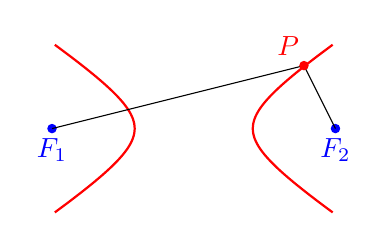
\begin{tikzpicture}	
		\def\a{1.5}	
		\def\b{1}			
		 \draw[scale=0.5,domain=-1.5:1.5,smooth,variable=\t,red,thick]
		  plot ({\a*cosh(\t )},{\b*sinh(\t)});
		   \draw[scale=0.5,domain=-1.5:1.5,smooth,variable=\t,red,thick]
		  plot ({-\a*cosh(\t )},{\b*sinh(\t)});
		\draw[fill,blue] (1.8,0) circle (1.5pt);
		\draw[fill,blue] (-1.8,0) circle (1.5pt);   
		\node[below,blue] at (1.8,0) {$F_2$};
		\node[below,blue] at (-1.8,0) {$F_1$};
		\node[above,red] at (1.2,0.8) {$P$};
%		
		\draw (-1.8,0) -- (1.4,0.8) --(1.8,0);
		\draw[fill,red] (1.4,0.8) circle (1.5pt);
		\end{tikzpicture}
	\end{center}
	
\end{frame}


\begin{frame}[label=conicas]{Notação}
	\begin{minipage}{0.4\textwidth}
		\begin{itemize}
			\item<1-> $F_1, F_2$: focos
			\item<2-> $F_1F_2$: segmento focal
			\item<3-> eixo focal
			\item<4-> $O$: centro da Hipérbole
			\item<5-> $A_1,A_2:$ Vértices
			\item<6-> $d(F_1,F_2)$: amplitude ou distância focal
		\end{itemize}
	\end{minipage}
	\begin{minipage}{0.5\textwidth}
		\begin{center}
			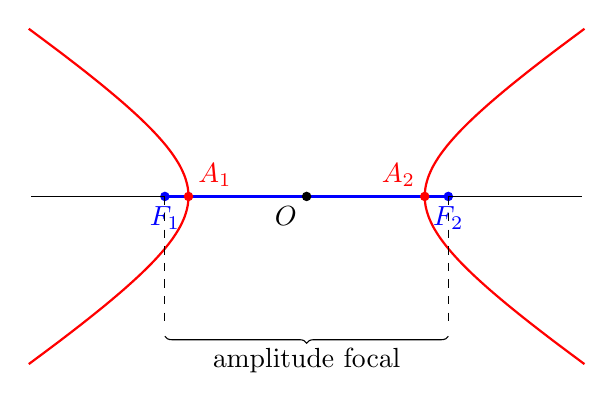
\begin{tikzpicture}
				\def\a{1.5}	
			\def\b{1}			
		
		
			%		
%			\draw (-1.8,0) -- (1.4,0.8) --(1.8,0);
%			\draw[fill,red] (1.4,0.8) circle (1.5pt);
	\uncover<1->{	\draw[scale=1,domain=-1.5:1.5,smooth,variable=\t,red,thick]
	plot ({\a*cosh(\t )},{\b*sinh(\t)});
	\draw[scale=1,domain=-1.5:1.5,smooth,variable=\t,red,thick]
	plot ({-\a*cosh(\t )},{\b*sinh(\t)});
	\draw[fill,blue] (1.8,0) circle (1.5pt);
	\draw[fill,blue] (-1.8,0) circle (1.5pt);   
	\node[below,blue] at (1.8,0) {$F_2$};
	\node[below,blue] at (-1.8,0) {$F_1$};
}
					\uncover<3->{	\draw (-3.5,0) -- (3.5,0);
					}	
			\uncover<2->{	
				\draw[thick,blue] (-1.8,0)--(1.8,0);  }
						
			\uncover<4->{	\node[below left] at (0,0) {$O$};
				\draw[fill] (0,0) circle (1.5pt);}
		%	\uncover<5->{	\draw (0,-1.5) -- (0,1.5);}
			%		\node[below right] at (2.5,0) {$x$};
			%		\node[above left] at (0,1.5) {$y$};		
		
			\uncover<5->{\draw[fill,red] (\a,0) circle (1.5pt);   	
				\draw[fill,red] (-\a,0) circle (1.5pt);
%				\draw[fill,red] (0,1) circle (1.5pt);   	
%				\draw[fill,red] (0,-1) circle (1.5pt);
				\node[above left,red] at (\a,0) {$A_2$};
				\node[above right,red] at (-\a,0) {$A_1$};
%				\node[left] at (0,1.2) {$B_2$};
%				\node[left] at (0,-1.2) {$B_1$};
}
		
			%	\draw (0,1) -- (1.3,0);
			\uncover<6->{\draw[decoration={brace,mirror,raise=5pt},decorate] (-1.8,-1.6)--(1.8,-1.6);
				\draw[dashed] (-1.8,0) -- (-1.8,-1.6);
				\draw[dashed] (1.8,0) -- (1.8,-1.6); 
				\node[below] at (0,-1.8) {amplitude focal};}	
%			\uncover<7->{\draw[decoration={brace,mirror,raise=5pt},decorate] (2.5,-1)--(2.5,1);
%				\draw[dashed] (0,-1) -- (2.5,-1);
%				\draw[dashed] (0,1) -- (2.5,1);
%				\node at (4,0) {eixo menor};}	
			
			
			
			%	\node at (-5,2) {$A_1,A_2,B_1,B_2:$ Vétices};
			
			%\node[above,red] at (1.2,0.8) {$P$};
			
			%\draw (-1.7,0) -- (1.2,0.8) --(1.7,0);
			%\draw[fill,red] (1.2,0.8) circle (1.5pt);
			\end{tikzpicture}
		\end{center}
	\end{minipage}
	
	%\end{scriptsize}
\end{frame}



\begin{frame}[label=conicas]
		\uncover<1->{\begin{block}{}
			Dado uma hipérbole, considere um sistema de eixos cartesianos tomando-se  $OX$ como o eixo focal e a origem como o centro da hipérbole. Neste caso, sendo $2c$ a distância focal,  $2a$ o valor absoluto da diferença das distâncias de um ponto qualquer da hipérbole aos focos, onde $0<a<c$ e $c^2=b^2+a^2$, então a equação da hipérbole é dada por
			
			\begin{center}
				\textcolor{red}{\fbox{$\displaystyle\frac{x^2}{a^2}-\frac{y^2}{b^2}=1$}}
			\end{center}
	\end{block}}

	\begin{center}
	%		%	\pgfmathsetmacro{\a}{1}
	%		\pgfmathsetmacro{\b}{2}	
	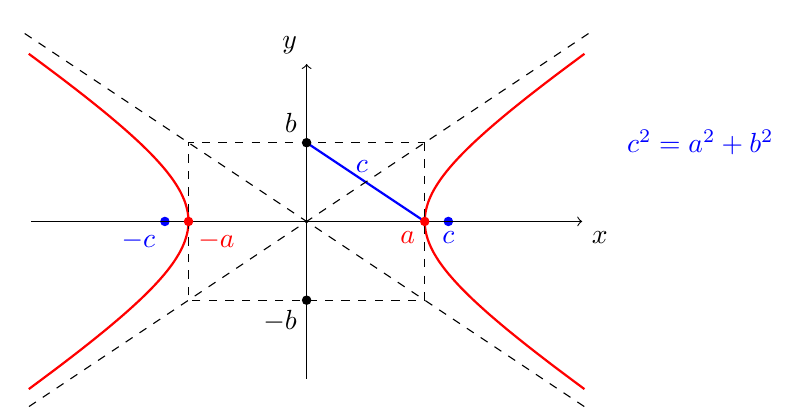
\begin{tikzpicture}	
	\def\a{1.5}	
	\def\b{1}			
	
	
	\coordinate (AB) at (\a,\b);
	\coordinate (ABm) at (-\a,-\b);
	\coordinate (mAB) at (-\a,\b);
		\coordinate (AmB) at (\a,-\b);
	
	
	\draw[domain=-1.5:1.5,smooth,variable=\t,red,thick]
	plot ({\a*cosh(\t )},{\b*sinh(\t)});
	\draw[domain=-1.5:1.5,smooth,variable=\t,red,thick]
	plot ({-\a*cosh(\t )},{\b*sinh(\t)});
	\draw[fill,blue] (1.8,0) circle (1.5pt);
	\draw[fill,blue] (-1.8,0) circle (1.5pt);   
	\node[below,blue] at (1.8,0) {$c$};
	\node[below left,blue] at (-1.8,0) {$-c$};
		
	
	
	\uncover<1->{	\draw[->] (-3.5,0) -- (3.5,0);
}	
\draw[blue,thick] (0,\b) -- (\a,0);
\node[blue] at (0.7,0.7) {$c$};
	\uncover<1->{	\draw[->] (0,-2.) -- (0,2);}
		\node[below right] at (3.5,0) {$x$};
		\node[above left] at (0,2) {$y$};
		
		
		
		\draw [shorten >= -2.5cm, shorten <=-2.5cm,dashed] (AB)--(ABm);
		\draw [shorten >= -2.5cm, shorten <=-2.5cm,dashed] (mAB)--(AmB);
		\draw[dashed] (AB) -- (AmB) -- (ABm) -- (mAB) -- (AB);
		
		
			\draw[fill,red] (\a,0) node[below left] {$a$} circle (1.5pt);
		\draw[fill,red] (-\a,0) node[below right] {$-a$} circle (1.5pt);
		
			\draw[fill] (0,\b) node[above left] {$b$} circle (1.5pt);
		\draw[fill] (0,-\b) node[below left] {$-b$} circle (1.5pt);
			
\node[blue] at (5,1) {$c^2=a^2+b^2$};



	\end{tikzpicture}
\end{center}
\end{frame}



\begin{frame}[label=conicas]
	\begin{minipage}{0.5\textwidth}
		\begin{obs}
 No caso em que os focos estiverem sobre o eixo $y$, a equação terá uma forma semelhante, com o sinal de menos acompanhando o termo com $x$ e consequentemente interceptará o eixo $y$ em $y=b$ e $y=-b$
	\end{obs}
	\end{minipage}
	\begin{minipage}{0.4\textwidth}
			\begin{center}
		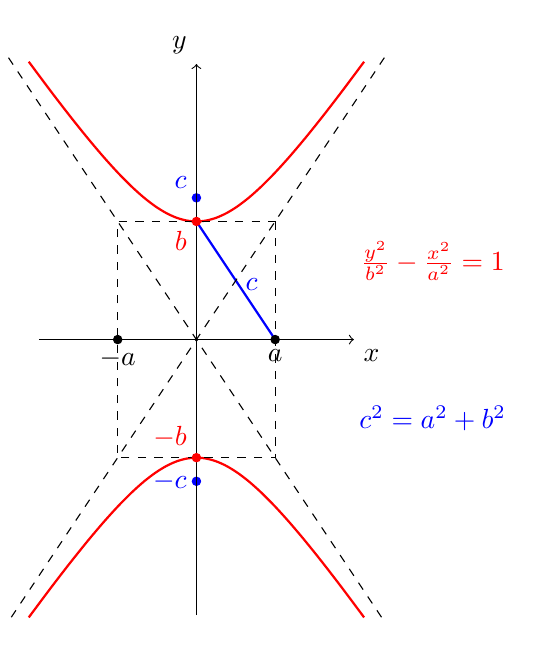
\begin{tikzpicture}	
	\def\a{1.5}	
	\def\b{1}		
	
		
	\coordinate (AB) at (\b,\a);
	\coordinate (ABm) at (-\b,-\a);
	\coordinate (mAB) at (-\b,\a);
	\coordinate (AmB) at (\b,-\a);		
	
	\draw[domain=-1.5:1.5,smooth,variable=\t,red,thick]
	plot ({\b*sinh(\t)},{\a*cosh(\t )});
	\draw[domain=-1.5:1.5,smooth,variable=\t,red,thick]
	plot ({\b*sinh(\t)},{-\a*cosh(\t )});
	\draw[fill,blue] (0,1.8) circle (1.5pt);
	\draw[fill,blue] (0,-1.8) circle (1.5pt);   
	\node[above left,blue] at (0,1.8) {$c$};
	\node[left,blue] at (0,-1.8) {$-c$};
	
	
	
	\uncover<1->{	\draw[->] (0,-3.5) -- (0,3.5);
	}	
	\draw[blue,thick] (0,\a) -- (\b,0);
	\node[blue] at (0.7,0.7) {$c$};
	\uncover<1->{	\draw[->] (-2,0) -- (2,0);}
	\node[below right] at (2,0) {$x$};
	\node[above left] at (0,3.5) {$y$};
	
	
		
	\draw [shorten >= -2.5cm, shorten <=-2.5cm,dashed] (AB)--(ABm);
	\draw [shorten >= -2.5cm, shorten <=-2.5cm,dashed] (mAB)--(AmB);
	\draw[dashed] (AB) -- (AmB) -- (ABm) -- (mAB) -- (AB);
	
	
	
	\draw[fill,red] (0,\a) node[below left] {$b$} circle (1.5pt);
	\draw[fill,red] (0,-\a) node[above left] {$-b$} circle (1.5pt);
	
	\draw[fill] (\b,0) node[below] {$a$} circle (1.5pt);
	\draw[fill] (-\b,0) node[below] {$-a$} circle (1.5pt);
	
	\node[red] at (3,1) {$\frac{y^2}{b^2}-\frac{x^2}{a^2}=1$};
	
	\node[blue] at (3,-1) {$c^2=a^2+b^2$};
	\end{tikzpicture}
\end{center}
	\end{minipage}

\end{frame}



\begin{frame}[label=conicas]
	\begin{exe}
		Determine os vértices e focos das hipérboles abaixo e faça um esboço.
		\begin{enumerate}
			\item $5x^2-9y^2=45$
			\item $\frac{9x^2}{25}-y^2+9=0$.
			
			\item A distância focal é $\sqrt{20}$, os focos pertencem ao eixo $OX$ e uma das assíntotas tem equação $y+3x=0$.
		\end{enumerate}
	\end{exe}
	
	
\end{frame}

\begin{frame}[label=conicas]
	
	\begin{casa}
	\begin{enumerate}
		\item 	Determine os vértices e focos da hipérboles $9x^2-4y^2=36$ abaixo e faça um esboço.
		
			\item Obtenha a equação da hipérbole cujos vértices são $(0,2)$ e $(0,-2)$ e os focos são $(0,3)$ e $(0,-3)$.
	\end{enumerate}
	\end{casa}
	
\end{frame}


%%%%%%%%%%%%%%%%%%%%%%%%%%%%%%%%%%%%%%%%%%%%%%%%%%%%%%%%%%%%%%%%%

\subsection*{Parábola}



\begin{frame}[label=conicas]{Parábola}
	%\begin{scriptsize}
	\begin{defin}[Parábola]
		Dados uma reta $\ell$  e um ponto $F$ não pertencente a $\ell$ no plano. Uma \dest{parábola} é o lugar geométrico dos pontos do plano equidistantes da reta $\ell$ e do ponto $F$. 
	\end{defin}
	\begin{center}
%		%	\pgfmathsetmacro{\a}{1}
%		\pgfmathsetmacro{\b}{2}	
		\begin{tikzpicture}	
		\def\a{1.5}	
		\def\b{1}			
		 \draw[scale=1,domain=-1.5:1.5,smooth,variable=\t,red,thick]
		  plot ({\t},{\t*\t});
		  \draw[fill,blue] (0,0.25) circle (1.5pt);
			\node[above,blue] at (0,0.25) {$F$};
	
%		
		\draw (-3,-0.25) -- (3,-.25) node[below right] {$\ell$};
		\draw[fill,red] (1,1) circle (1.5pt);
			\node[right,red] at (1,1) {$P$};
		\end{tikzpicture}
	\end{center}
	
\end{frame}


\begin{frame}[label=conicas]{Notação}
	\begin{minipage}{0.4\textwidth}
		\begin{itemize}
			\item<2-> $F$: focos
			\item<3-> $\ell$: diretriz
			\item<4-> eixo da parábola
			\item<5-> $V$: vértice
			
		\end{itemize}
	\end{minipage}
	\begin{minipage}{0.5\textwidth}
	\begin{center}
		%		%	\pgfmathsetmacro{\a}{1}
		%		\pgfmathsetmacro{\b}{2}	
		\begin{tikzpicture}	
		
		\onslide<1->{\draw[scale=1,domain=-1.5:1.5,smooth,variable=\t,red,thick]
		plot ({\t},{\t*\t});}
		\onslide<2->{\draw[fill,blue] (0,0.25) circle (1.5pt);
		\node[above right,blue] at (0,0.25) {$F$};}
		\onslide<3->{\draw[thick] (-3,-0.25) -- (3,-.25) node[below right] {$\ell$};}
		\onslide<4->{\draw[thick] (0,-1) -- (0,3); }
		\onslide<5->{\draw[fill,red] (0,0) circle (1.5pt);
		\node[below right,red] at (0,0) {$V$};}
		\end{tikzpicture}
	\end{center}
	\end{minipage}
	
	%\end{scriptsize}
\end{frame}


\begin{frame}[label=conicas]
	
	\uncover<1->{\begin{block}{}
		Dado uma parábola, considere um sistema de eixos cartesianos com a origem $O$ no vértice da parábola e eixo $OY$ determinado pelo eixo da parábola de tal modo que o foco pertença ao semi-eixo positivo. Neste caso, sendo $2p$ a distância de $F$ a $\ell$, então a equação da parábola é dada por
		
		\begin{center}
			\textcolor{red}{\fbox{$\displaystyle x^2=4py$}}
		\end{center}
\end{block}}

\begin{center}
	%		%	\pgfmathsetmacro{\a}{1}
	%		\pgfmathsetmacro{\b}{2}	
	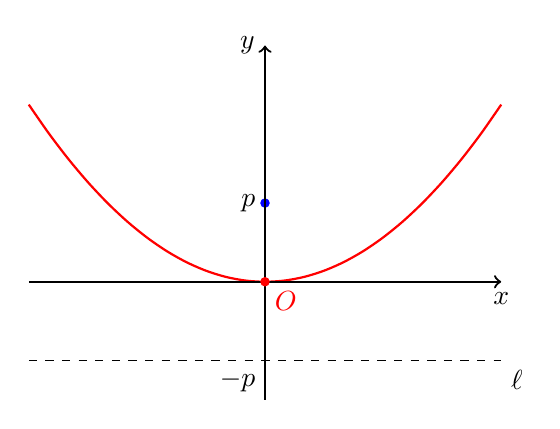
\begin{tikzpicture}	
		\def\p{1}	
	\onslide<1->{\draw[scale=1,domain=-3:3,smooth,variable=\t,red,thick]
		plot ({\t},{\t*\t/(4*\p)});}
	\onslide<1->{\draw[fill,blue] (0,\p) circle (1.5pt);}
%		\node[above right,blue] at (0,\p) {$F$};
	\draw[thick,->] (-3,0) -- (3,0) node[below] {$x$};
	\onslide<1->{\draw[dashed] (-3,-\p) -- (3,-\p) node[below right] {$\ell$};}
	\onslide<1->{\draw[thick,->] (0,-1.5) -- (0,3) node[left] {$y$}; }
	\onslide<1->{\draw[fill,red] (0,0) circle (1.5pt);
		\node[below right,red] at (0,0) {$O$};}
	\node[below left] at (0,-\p) {$-p$};
		\node[ left] at (0,\p) {$p$};
	\end{tikzpicture}
\end{center}

%\end{scriptsize}
\end{frame}

\begin{frame}[label=conicas]
	
	\uncover<1->{\begin{obs}
		Se o sistema de eixos for escolhido com de tal modo que o foco pertença ao semi-eixo \dest{negativo} de $OY$, então a equação da parábola é dada por
			
			\begin{center}
				\textcolor{red}{\fbox{$\displaystyle x^2=-4py$}}
			\end{center}
	\end{obs}}
	
	\begin{center}
		%		%	\pgfmathsetmacro{\a}{1}
		%		\pgfmathsetmacro{\b}{2}	
		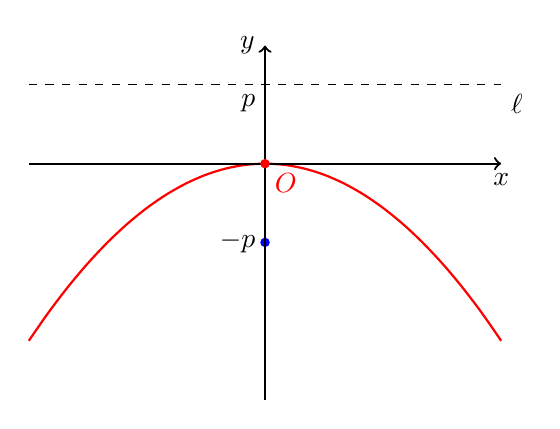
\begin{tikzpicture}	
		\def\p{1}	
		\onslide<1->{\draw[scale=1,domain=-3:3,smooth,variable=\t,red,thick]
			plot ({\t},{-\t*\t/(4*\p)});}
		\onslide<1->{\draw[fill,blue] (0,-\p) circle (1.5pt);}
		%		\node[above right,blue] at (0,\p) {$F$};
		\draw[thick,->] (-3,0) -- (3,0) node[below] {$x$};
		\onslide<1->{\draw[dashed] (-3,\p) -- (3,\p) node[below right] {$\ell$};}
		\onslide<1->{\draw[thick,->] (0,-3) -- (0,1.5) node[left] {$y$}; }
		\onslide<1->{\draw[fill,red] (0,0) circle (1.5pt);
			\node[below right,red] at (0,0) {$O$};}
		\node[below left] at (0,\p) {$p$};
		\node[ left] at (0,-\p) {$-p$};
		\end{tikzpicture}
	\end{center}
	
	%\end{scriptsize}
\end{frame}

\begin{frame}[label=conicas]
	
	\uncover<1->{\begin{obs}
				
			Se o sistema de eixos for escolhido com o eixo $OX$ sendo o eixo da parábola teremos as seguintes situações.
				\end{obs}}
	
		
	\begin{minipage}{0.4\textwidth}
		\begin{center}
		%		%	\pgfmathsetmacro{\a}{1}
		%		\pgfmathsetmacro{\b}{2}	
		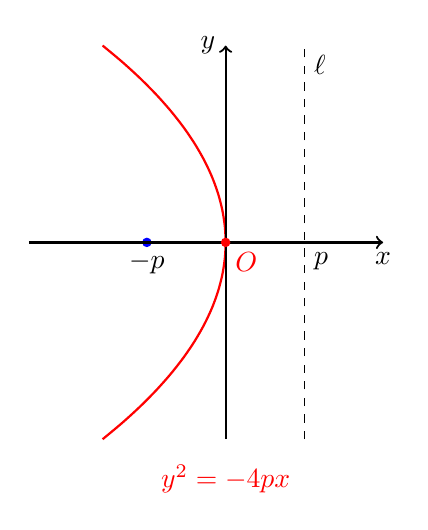
\begin{tikzpicture}	
		\def\p{1}	
		\onslide<1->{\draw[scale=1,domain=-2.5:2.5,smooth,variable=\t,red,thick]
			plot ({-\t*\t/(4*\p)},{\t});}
		\onslide<1->{\draw[fill,blue] (-\p,0) circle (1.5pt);}
		%		\node[above right,blue] at (0,\p) {$F$};
		\draw[thick,->] (-2.5,0) -- (2,0) node[below] {$x$};
		\onslide<1->{\draw[dashed] (\p,-2.5) -- (\p,2.5) node[below right] {$\ell$};}
		\onslide<1->{\draw[thick,->] (0,-2.5) -- (0,2.5) node[left] {$y$}; }
		\onslide<1->{\draw[fill,red] (0,0) circle (1.5pt);
			\node[below right,red] at (0,0) {$O$};}
		\node[below right] at (\p,0) {$p$};
		\node[ below] at (-\p,0) {$-p$};
		\node[red] at (0,-3) {$y^2=-4px$};
		\end{tikzpicture}
	\end{center}
	\end{minipage}
\begin{minipage}{0.4\textwidth}
	\begin{center}
		%		%	\pgfmathsetmacro{\a}{1}
		%		\pgfmathsetmacro{\b}{2}	
		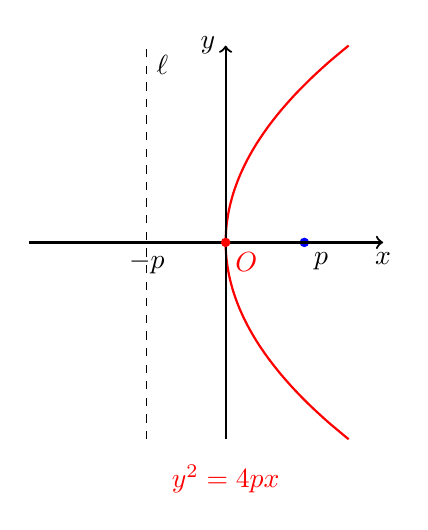
\begin{tikzpicture}	
		\def\p{1}	
		\onslide<1->{\draw[scale=1,domain=-2.5:2.5,smooth,variable=\t,red,thick]
			plot ({\t*\t/(4*\p)},{\t});}
		\onslide<1->{\draw[fill,blue] (\p,0) circle (1.5pt);}
		%		\node[above right,blue] at (0,\p) {$F$};
		\draw[thick,->] (-2.5,0) -- (2,0) node[below] {$x$};
		\onslide<1->{\draw[dashed] (-\p,-2.5) -- (-\p,2.5) node[below right] {$\ell$};}
		\onslide<1->{\draw[thick,->] (0,-2.5) -- (0,2.5) node[left] {$y$}; }
		\onslide<1->{\draw[fill,red] (0,0) circle (1.5pt);
			\node[below right,red] at (0,0) {$O$};}
		\node[below right] at (\p,0) {$p$};
		\node[ below] at (-\p,0) {$-p$};
		\node[red] at (0,-3) {$y^2=4px$};
		\end{tikzpicture}
	\end{center}
\end{minipage}
	
	%\end{scriptsize}
\end{frame}

\begin{frame}[label=conicas]{Curvas que não são parábolas}
	\begin{enumerate}
		\item $y=x^4$
		\item $y=\cosh x=\frac{e^x+e^{-x}}{2}$  ( catenária ) 
	\end{enumerate}
	
	
	Quando um cabo flexível pesado é suspenso entre dois pontos  na mesma altura, vemos a formação de uma curva conhecida como \dest{catenária}, do latim \textit{catena} que significa corrente. 
	\begin{figure}
		\includegraphics[scale=0.5]{figuras/catenaria.png}
		\caption{Kette Kettenkurve Catenary, Kamel15}
	\end{figure}
	
\end{frame}


\begin{frame}[label=conicas]{Por que o gráfico de uma função do $2^\circ$ é uma parábola?}
\begin{block}{Função do $2^\circ$ grau}
	\[f(x)=ax^2+bx+c, \ a\neq 0.\]
	\[y=ax^2+bx+c\]
\end{block}

\begin{exe}
\begin{enumerate}
\item Esboce a parábola $y=2x^2$, determine seu foco e a equação da reta 
diretriz
\item Use o item anterior para esboçar o gráfico de  $y=2x^2-12x+17$.
\end{enumerate}
\end{exe}

%Em particular, se $b=c=0$ e $a=1/4p$ temos que 
%\[y=\frac{1}{4p}x^2\Rightarrow x^2=4py.\]
\end{frame}





\begin{frame}[label=conicas]{Parábola com foco no eixo $OY$}
	\begin{minipage}{0.5\textwidth}
\begin{center}
	%		%	\pgfmathsetmacro{\a}{1}
	%		\pgfmathsetmacro{\b}{2}	
	\begin{tikzpicture}	
	\def\p{1}	
	\onslide<1->{\draw[scale=1,domain=-3:3,smooth,variable=\t,red,thick]
		plot ({\t},{\t*\t/(4*\p)});}
	\onslide<1->{\draw[fill,blue] (0,\p) circle (1.5pt);}
	%		\node[above right,blue] at (0,\p) {$F$};
	\draw[thick,->] (-3,0) -- (3,0) node[below] {$x$};
	\onslide<1->{\draw[dashed] (-3,-\p) -- (3,-\p) node[below right] {$\ell$};}
	\onslide<1->{\draw[thick,->] (0,-1.5) -- (0,3) node[left] {$y$}; }
	\onslide<1->{\draw[fill,red] (0,0) circle (1.5pt);
		\node[below right,red] at (0,0) {$O$};}
	\node[below left] at (0,-\p) {$-p$};
	\node[ left] at (0,\p) {$p$};
		\node[red] at (0,-3) {$x^2=4py$};
	\end{tikzpicture}
\end{center}
	\end{minipage}
	\begin{minipage}{0.3\textwidth}
	\begin{center}
		%		%	\pgfmathsetmacro{\a}{1}
		%		\pgfmathsetmacro{\b}{2}	
		\begin{tikzpicture}	
		\def\p{1}	
		\onslide<1->{\draw[scale=1,domain=-3:3,smooth,variable=\t,red,thick]
			plot ({\t},{-\t*\t/(4*\p)});}
		\onslide<1->{\draw[fill,blue] (0,-\p) circle (1.5pt);}
		%		\node[above right,blue] at (0,\p) {$F$};
		\draw[thick,->] (-3,0) -- (3,0) node[below] {$x$};
		\onslide<1->{\draw[dashed] (-3,\p) -- (3,\p) node[below right] {$\ell$};}
		\onslide<1->{\draw[thick,->] (0,-3) -- (0,1.5) node[left] {$y$}; }
		\onslide<1->{\draw[fill,red] (0,0) circle (1.5pt);
			\node[below right,red] at (0,0) {$O$};}
		\node[below left] at (0,\p) {$p$};
		\node[ left] at (0,-\p) {$-p$};
			\node[red] at (0,-4) {$x^2=-4py$};
		\end{tikzpicture}
	\end{center}
\end{minipage}
\end{frame}


\begin{frame}[label=conicas]{Parábola com foco no eixo $OX$}

\begin{minipage}{0.4\textwidth}
	\begin{center}
		%		%	\pgfmathsetmacro{\a}{1}
		%		\pgfmathsetmacro{\b}{2}	
		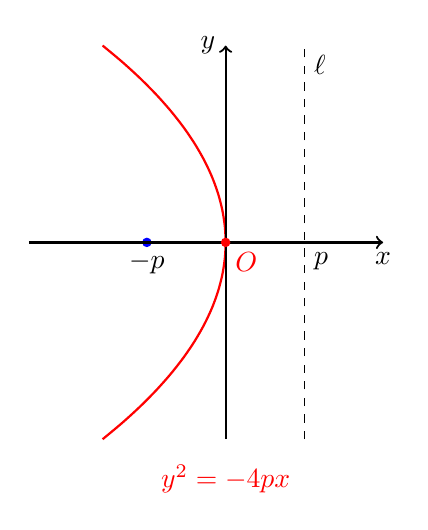
\begin{tikzpicture}	
		\def\p{1}	
		\onslide<1->{\draw[scale=1,domain=-2.5:2.5,smooth,variable=\t,red,thick]
			plot ({-\t*\t/(4*\p)},{\t});}
		\onslide<1->{\draw[fill,blue] (-\p,0) circle (1.5pt);}
		%		\node[above right,blue] at (0,\p) {$F$};
		\draw[thick,->] (-2.5,0) -- (2,0) node[below] {$x$};
		\onslide<1->{\draw[dashed] (\p,-2.5) -- (\p,2.5) node[below right] {$\ell$};}
		\onslide<1->{\draw[thick,->] (0,-2.5) -- (0,2.5) node[left] {$y$}; }
		\onslide<1->{\draw[fill,red] (0,0) circle (1.5pt);
			\node[below right,red] at (0,0) {$O$};}
		\node[below right] at (\p,0) {$p$};
		\node[ below] at (-\p,0) {$-p$};
		\node[red] at (0,-3) {$y^2=-4px$};
		\end{tikzpicture}
	\end{center}
\end{minipage}
\begin{minipage}{0.3\textwidth}
	\begin{center}
		%		%	\pgfmathsetmacro{\a}{1}
		%		\pgfmathsetmacro{\b}{2}	
		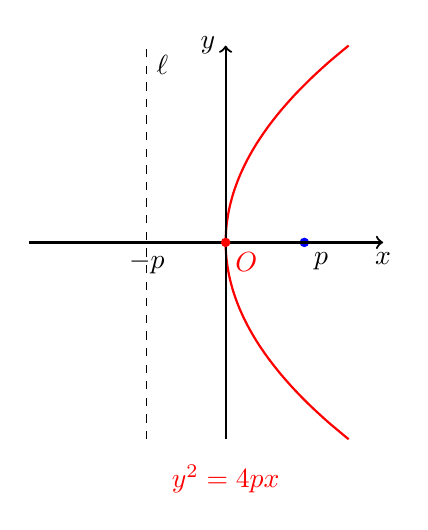
\begin{tikzpicture}	
		\def\p{1}	
		\onslide<1->{\draw[scale=1,domain=-2.5:2.5,smooth,variable=\t,red,thick]
			plot ({\t*\t/(4*\p)},{\t});}
		\onslide<1->{\draw[fill,blue] (\p,0) circle (1.5pt);}
		%		\node[above right,blue] at (0,\p) {$F$};
		\draw[thick,->] (-2.5,0) -- (2,0) node[below] {$x$};
		\onslide<1->{\draw[dashed] (-\p,-2.5) -- (-\p,2.5) node[below right] {$\ell$};}
		\onslide<1->{\draw[thick,->] (0,-2.5) -- (0,2.5) node[left] {$y$}; }
		\onslide<1->{\draw[fill,red] (0,0) circle (1.5pt);
			\node[below right,red] at (0,0) {$O$};}
		\node[below right] at (\p,0) {$p$};
		\node[ below] at (-\p,0) {$-p$};
		\node[red] at (0,-3) {$y^2=4px$};
		\end{tikzpicture}
	\end{center}
\end{minipage}
\end{frame}


\begin{frame}[label=conicas]
\begin{exe}
	\begin{enumerate}
		\item Determine o foco  e a equação da reta diretriz das parábolas abaixo e faça um esboço:
		\begin{enumerate}[a]
			\item $y=10x^2$
			\item $y^2=5x$
		\end{enumerate}
		
		\item Obtenha a equação da parábola de vértice em $(0,0)$ e foco em $(-8,0)$.
	\end{enumerate}
\end{exe}


\end{frame}


\begin{frame}[label=conicas]
	\begin{casa}
		
		\begin{enumerate}
			\item Determine o foco, uma equação da diretriz e faça um esboço da parábola
			\[y^2=4x\]
			
			\item Obtenha a equação da parábola de vértice em $(0,0)$ cuja diretriz tem equação $y=2$ e faça um esboço.
		\end{enumerate}
			
	\end{casa}
\end{frame}






